%==============================================================================
% Document header
%==============================================================================
\documentclass[a4paper,11pt]{article}

% Margin setup to use more of the page
\usepackage[top=3cm, bottom=3cm, left=2cm, right=2cm]{geometry}

% Color package
\usepackage[usenames,dvipsnames,table]{xcolor}

% Hyperrefs
\usepackage[
  colorlinks = true,
  linkcolor  = black,
  citecolor  = black,
  urlcolor   = blue
]{hyperref}

% Longtable
\usepackage{longtable}

% Graphics, multirow
\usepackage{graphicx}
\usepackage{multirow}

% Appendix package
\usepackage[toc,page]{appendix}

% Configure header
\usepackage{fancyhdr}
\setlength{\headheight}{15.2pt}
\pagestyle{fancy}
\fancyhead[L]{\nouppercase{\leftmark}}
\fancyhead[R]{}
\renewcommand{\footrulewidth}{0.4pt}

% Row number command
\newcounter{rownr}
\newcommand{\rownumber}{\stepcounter{rownr}\arabic{rownr}}

%==============================================================================
% Start of document
%==============================================================================
\begin{document}

%------------------------------------------------------------------------------
% Title
%------------------------------------------------------------------------------
\begin{titlepage}

\begin{figure}[h]
  
\includegraphics[height=3cm]{fig/kth-logo}
\end{figure}

\vspace*{3cm}

%---------------------------------------------------------------
% name
%---------------------------------------------------------------
\noindent{\Large \textbf{IUB power-on and temperature sensor readout protocol}}

\noindent \rule{\textwidth}{.1cm}

\hfill 2016-03-15

\vfill

%---------------------------------------------------------------
% name
%---------------------------------------------------------------
\noindent {\Large \textbf{Theodor-Adrian Stana (KTH Particle and Astroparticle Physics)}}

\noindent \rule{\textwidth}{.05cm}

\end{titlepage}


%------------------------------------------------------------------------------
% Licensing info
%------------------------------------------------------------------------------
\pagebreak

\thispagestyle{empty}

\addcontentsline{toc}{section}{Licensing information}
\section*{Licensing information}

\noindent
This document is licensed under a Creative Commons Attribution-ShareAlike 4.0
International License. If you have not received a copy of the license along with this
work, see \\
\url{http://creativecommons.org/licenses/by-sa/4.0/}

%------------------------------------------------------------------------------
% Revision history
%------------------------------------------------------------------------------
\section*{Revision history}
\addcontentsline{toc}{section}{Revision history}

\centerline
{
  \rowcolors{2}{white}{gray!25}
  \begin{tabular}{l c p{.6\textwidth}}
  \hline
  \multicolumn{1}{c}{\textbf{Date}} & \multicolumn{1}{c}{\textbf{Version}} & \multicolumn{1}{c}{\textbf{Change}} \\
  \hline
  2016-03-15 & 1.0 & First draft \\
  \hline
  \end{tabular}
}

%------------------------------------------------------------------------------
% Table of contents, list of figs, tables
%------------------------------------------------------------------------------
\pagebreak
\pdfbookmark[1]{\contentsname}{toc}
\tableofcontents

\listoffigures
\listoftables

%------------------------------------------------------------------------------
% List of abbreviations
%------------------------------------------------------------------------------
\pagebreak
\section*{List of abbreviations}
\begin{tabular}{l l}
CPLD & Complex Programmable Logic Device \\
DAQ & Data Acquisition \\
DIO & Digital Input/Output (board) \\
FADC & Flash Analog-to-Digital (board) \\
IUB & Interface Utility Board \\
MPB & Main Processing Board \\
PCU & Payload Control Unit \\
PMT & Photo-Multiplier Tube \\
PVA & Pressure Vessel Assembly \\
\end{tabular}
\addcontentsline{toc}{section}{List of abbreviations}

%==============================================================================
% SEC: Intro
%==============================================================================
\pagebreak
\section{Introduction}
\label{sec:intro}

This document describes the protocol and hardware used for powering up boards in the
PoGO+ DAQ system inside the PVA electronics crate.

Figure~\ref{fig:bd-polarimeter-electronics} shows a block diagram of the PVA electronics
crate. Among the various boards present in the system, an IUB (Interface Utility 
Board) developed by DST Control in Link\"{o}ping, Sweden, communicates to a Minion 
board for several purposes:

\begin{itemize}
  \item enable/disable 5~V power to several boards in the system
  \item enable/disable 12~V power to the PMTs
  \item obtain the readings of temperature sensors multiplexed on the Minion board
\end{itemize}

Several 5~V and 12~V power lines arrive to the Power Board from the DC/DC converter in the 
PCU crate. The Power Board drives the power lines to power on enabled boards in the DAQ 
system.

As can be seen in Figure~\ref{fig:pow-cmd-functioning}, power-up is performed by running 
the "\verb=pow=" command in the \verb=PC= (Power Control) program on the PC/104 flight
computer. The command initiates a connection to the MPB inside the PCU crate and the MPB 
forwards the command to the IUB inside the PVA crate over a so-called RSPI protocol. The 
PVA crate IUB interprets this RSPI command and translates it to a set of three RS-422 
signals (\verb=SHIFT=, \verb=READ=, \verb=DATA= -- see Section~\ref{sec:prot}) that are 
sent to the Minion. The Minion interprets these signals and assigns enable outputs to the 
Power Board, which then drives voltages to the enabled devices as appropriate.

Sixteen temperature sensors placed in the PVA electronics crate and in the polarimeter
itself are connected to the Minion. The readings from these sensors are multiplexed and 
sent out to the IUB.

\begin{figure}[h]
  \centerline{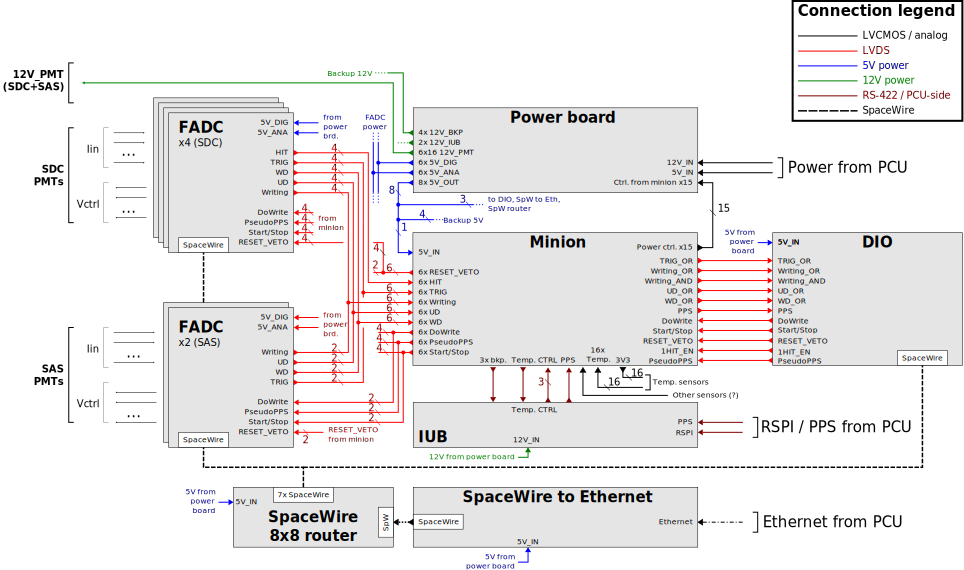
\includegraphics[width=\textwidth]{fig/bd-polarimeter-electronics}}
  \caption{\label{fig:bd-polarimeter-electronics} Electronics in the PVA crate}
\end{figure}

\begin{figure}[h]
  \centerline{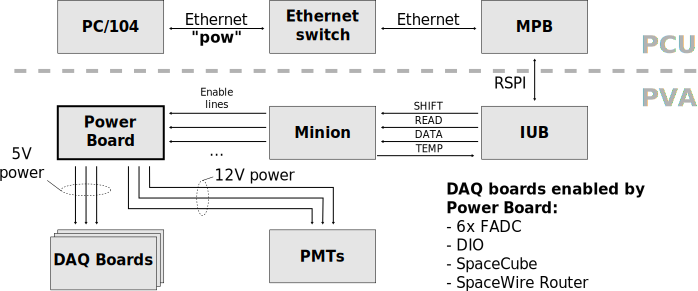
\includegraphics[width=\textwidth]{fig/pow-cmd-functioning}}
  \caption{\label{fig:pow-cmd-functioning} DAQ system power-on chain}
\end{figure}

%==============================================================================
% SEC: Protocol
%==============================================================================
\pagebreak
\section{IUB to Minion protocol}
\label{sec:prot}

Three RS-422 signals are continously driven by the IUB:

\begin{itemize}
  \item \verb=DATA= -- Data to be interpreted by the Minion
  \item \verb=SHIFT= -- Clock signal for shifting in bits on the \verb=DATA= line
  \item \verb=READ= -- Signals the start of the bit pattern on the \verb=DATA= line
\end{itemize}

A number of forty bits are sent out by the IUB on the \verb=DATA= line. As shown in
Figure~\ref{fig:protocol}, the start of the bit pattern is signaled by asserting
the \verb=READ= signal. A high \verb=READ= signal indicates bit 0 of the \verb=DATA=
pattern. Bits on the \verb=DATA= line are issued in big endian format, i.e., the first
is bit 0, followed by bit 1, bit 2, etc., and ending with bit 39. All forty \verb=DATA= 
bits and the \verb=READ= signal are issued on the rising edge of \verb=SHIFT= and are 
stable on the falling edge thereof.

Table~\ref{tbl:bits} shows the used bits in the \verb=DATA= pattern. The first four
bits in the pattern tell the Minion which temperature sensor the IUB will read out.
These bits are used by the Minion as a selection signal for a temperature sensor 
multiplexer implemented in gateware. The IUB reads all temp sensors in sequence: it reads
the first sensor on the first 40-bit \verb=DATA= pattern, the second sensor on the second 
40-bit \verb=DATA= pattern, ends with the sixteenth and then reads the first again.

The rest of the bits in the \verb=DATA= pattern are used to power boards on and off. A 
high bit signals the board should be powered on.

\begin{figure}[h]
  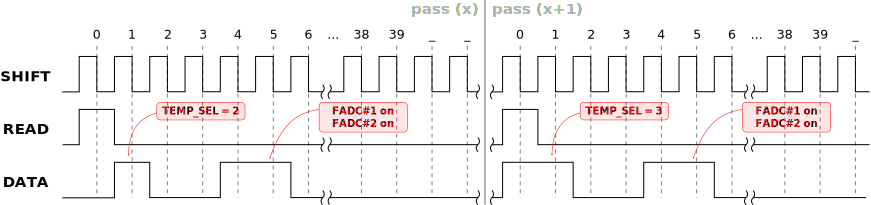
\includegraphics[width=.92\textwidth]{fig/protocol}
  \caption{\label{fig:protocol} Power-on and temperature control protocol from the IUB
    to the Minion}
\end{figure}

\begin{table}[h]
  \caption{\label{tbl:bits} Used bits in the pattern on the DATA line}
  \centerline {
    \rowcolors{2}{white}{gray!25}
    \begin{tabular}{r p{.5\textwidth}}
      \hline
      \textbf{Bit} & \textbf{Description} \\
      \hline
      0 & Temperature selection -- bit 0 \\
      1 & Temperature selection -- bit 1 \\
      2 & Temperature selection -- bit 2 \\
      3 & Temperature selection -- bit 3 \\
      4 & Power on FADC\#1 \\
      5 & Power on FADC\#2 \\
      6 & Power on FADC\#3 \\
      7 & Power on FADC\#4 \\
      8 & Power on FADC\#5 \\
      9 & Power on FADC\#6 \\
      17 & Power on SpaceCube \\
      18 & Power on SpaceWire Router \\
      20 & Power on PMTs connected to FADC\#1 \\
      21 & Power on PMTs connected to FADC\#2 \\
      22 & Power on PMTs connected to FADC\#3 \\
      23 & Power on PMTs connected to FADC\#4 \\
      24 & Power on PMTs connected to FADC\#5 \\
      25 & Power on PMTs connected to FADC\#6 \\
      32 & Power on DIO \\
      \hline
    \end{tabular}
  }
\end{table}

\pagebreak
The bit pattern is sent out continuously by the IUB. After a delay of about 2~ms
after the bit 39 is sent, the bit pattern is sent again, this time with
an incremented value on the temperature selection bits, as can be seen in
Figure~\ref{fig:protocol}.  The roughly 2~ms delay between \verb=DATA= patterns is used by 
the IUB to read out the selected temperature sensor from the Minion. This readout is 
performed on a separate RS-422 line -- \verb=TEMP=, output by the Minion to the IUB.

%==============================================================================
% SEC: Minion gateware
%==============================================================================
\section{Minion gateware}
\label{sec:minion}

Gateware implemented in VHDL on the Minion's on-board CPLD receives the data pattern
from the IUB and acts upon it. Figure~\ref{fig:minion-hdl} shows a diagram of this
part of the Minion gateware.

\begin{figure}[b]
  \centerline{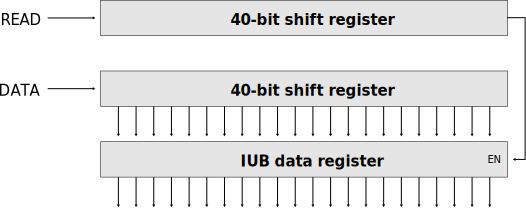
\includegraphics[width=.75\textwidth]{fig/minion-hdl}}
  \caption{\label{fig:minion-hdl} Diagram of Minion gateware handling IUB data stream}
\end{figure}

On each falling edge of the \verb=SHIFT= signal, the \verb=DATA= and the \verb=READ= line 
are clocked into a shift register. When the last bit of the shift register on the 
\verb=READ= line is high, the bits of the \verb=DATA= register are stored in parallel to 
another register. This register is used for processing, while the shift register is used 
for receiving the next bit pattern.

\begin{figure}
  \centerline{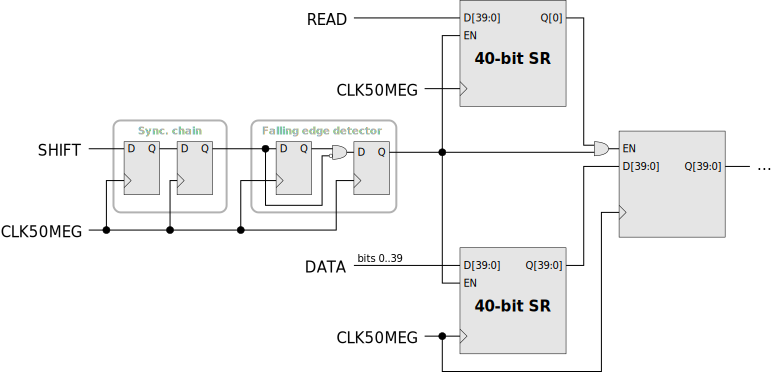
\includegraphics[width=.95\textwidth]{fig/minion-hdl-detail}}
  \caption{\label{fig:minion-hdl-detail} Detailed implementation of the Minion shift     
           registers}
\end{figure}

\begin{figure}[b]
  \centerline{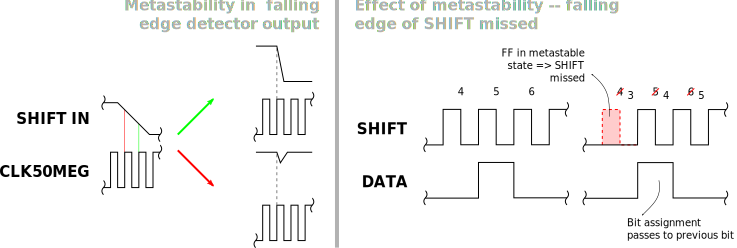
\includegraphics[width=\textwidth]{fig/missed-bit}}
  \caption{\label{fig:missed-bit} Missed bit due to metastability in SHIFT falling edge
  detector}
\end{figure}

To keep to good hardware design practices, a single clock is used within the design --
the Minion's on-board 50~MHz clock. The detailed implementation of this part of the
gateware is shown in Figure~\ref{fig:minion-hdl-detail}. A falling edge of the 
\verb=SHIFT= signal is used as an enable signal to the shift registers, which are clocked 
by the 50~MHz clock. Forty \verb=SHIFT= cycles after the \verb=READ= is received from the 
IUB, the last bit of the \verb=READ= signal's shift register will be high. At the same 
time, forty \verb=DATA= bits will have been received and the last bit of the \verb=READ= 
shift register is used to store the \verb=DATA= shift register for processing. 

Note how the \verb=SHIFT= signal is synchronized in the 50~MHz clock domain. This is
necessary as there may be occasions when a \verb=DATA= bit is "missed". This
can happen due to the first flip-flop in the falling edge detector of the \verb=SHIFT= 
signal being in a metastable state, which means it may
yield a high or a low output, depending on where the 50~MHz sampling clock hits. If
the output yields a low, a single-bit delay will appear forty-bit \verb=DATA= cycles, the 
effect of which is the power-on bit toggling in the Minion from one forty-bit cycle to
the next. This is shown in Figure~\ref{fig:missed-bit}.

%------------------------------------------------------------------------------
% SUBSEC: Minion gateware repository
%------------------------------------------------------------------------------
\subsection{Minion gateware repository}

The Minion gateware is stored online in a github repository. The interested reader can 
read the \textit{exact} gateware implementation by cloning the repository from the 
following address:

\begin{center}
  \url{https://github.com/tstana/minion-hdl}
\end{center}

%==============================================================================
% Bibliography
%==============================================================================
\pagebreak
%\bibliographystyle{ieeetr}
%\bibliography{daq-pow}
%\addcontentsline{toc}{section}{References}

\end{document}
